% Reviewer-driven WACV revision. Numerical placeholders must be replaced only
% from frozen, versioned experiment artifacts before submission.
\documentclass[10pt,twocolumn,letterpaper]{article}

\usepackage[review,applications]{wacv}
\usepackage{amsmath,amssymb,booktabs,multirow}
\usepackage{graphicx}
\usepackage{iftex}
\ifPDFTeX\else
  % Tectonic uses XeTeX locally; use the installed Times-compatible face.
  % Overleaf/pdfLaTeX continues to use the official WACV Times setup.
  \usepackage{fontspec}
  \setmainfont{Times New Roman}
\fi
\usepackage{microtype}
\usepackage{placeins}
\usepackage{xcolor}
\usepackage{enumitem}
\usepackage{mathtools}
\usepackage{pifont}
\usepackage{algorithm}
\usepackage{algpseudocode}
\usepackage{tikz}
\usetikzlibrary{arrows.meta,positioning,fit,calc,backgrounds}

% Visible draft markers prevent incomplete results from entering a submission.
\newcommand{\pending}[1]{\textcolor{red!75!black}{\textbf{[PENDING: #1]}}}
\newcommand{\pendingcell}{\textcolor{red!75!black}{--}}
\newcommand{\draftnote}[1]{\par\noindent\colorbox{yellow!20}{%
  \parbox{0.96\linewidth}{\textbf{Draft requirement:} #1}}\par}
\newcommand{\cmark}{\ding{51}}
\newcommand{\xmark}{\ding{55}}
\newcommand{\wacvtablefont}{\footnotesize}


\definecolor{wacvblue}{rgb}{0.21,0.49,0.74}
\usepackage[breaklinks,colorlinks,allcolors=wacvblue]{hyperref}

\def\wacvPaperID{2841}
\def\confName{WACV}
\def\confYear{2027}

\title{OrnaScout: Fixed-Budget Visual Evidence Allocation and Selective\\
Prediction for High-Resolution UAV Nursery Imagery}

\author{Anonymous WACV submission}

\begin{document}
\maketitle
\begin{abstract}
High-resolution UAV frames can contain hundreds of small nursery plants, yet compact vision--language models (VLMs) accept only a limited visual context. Whole-image downsampling removes instance evidence, while exhaustive overlapping tiles make multimodal inference scale poorly with image size. We formulate this mismatch as source-level prediction under a fixed budget of $K$ VLM calls. OrnaScout first applies a detector to candidate tiles, then allocates the budget among ranked evidence and spatially diverse exploration. A fixed-schema decoder produces auditable inventory-oriented records, an overlap-aware reducer combines accepted tile records, and a validation-only gate refers uncertain source decisions for human review. The evaluation uses source-disjoint Magnolia and Azalea imagery and compares detector-only aggregation, whole-image and uniformly tiled VLM inference, equal-budget routing policies, directed crop transfer, and selective-risk baselines. \pending{Insert only artifact-verified source-level utility, transfer, risk--coverage, and end-to-end efficiency findings.} The study is designed to determine when multimodal evidence adds value beyond detection and how foreground recall, spatial diversity, negative evidence, accepted risk, and compute trade off under crop shift.
\end{abstract}

\section{Introduction}
Nursery inventory from unmanned aerial vehicles (UAVs) is a high-resolution, small-object problem. A single RGB frame may contain many repeated plants, partial crowns, shadows, ground fabric, and row-edge truncation. A detector can localize annotated plants, but converting thousands of local responses into one auditable source-level record still requires decisions about where to inspect, how to reconcile overlapping evidence, and when the available evidence is insufficient. These decisions become more difficult when canopy geometry, plant density, and object scale change across crops.

Compact vision--language models (VLMs) offer a common interface for structured visual questions, but their visual context is poorly matched to 5K aerial frames. Whole-image downsampling can erase small instances; exhaustive tiling repeats overlapping regions and makes VLM cost grow with image size; and syntactically valid outputs can remain visually unsupported. Bounded inference is therefore not merely a deployment convenience: it determines which visual evidence can influence the final decision~\cite{kode2026drone}.

We study the following falsifiable problem. Given a source image and a fixed budget of at most $K$ VLM calls, which regions should be inspected, what source-level inventory record can be supported, and when should the system abstain? OrnaScout separates four responsibilities. A detector supplies inexpensive local evidence over all candidate tiles. A selector allocates the expensive VLM budget. A structured decoder and overlap-aware reducer produce one source record. A validation-fitted gate decides whether that record should be accepted or reviewed. The gate acts after generation and is evaluated as a safety mechanism, not as a source of VLM-call savings.

The agricultural scope is deliberately bounded. The available annotations support plant presence, count-oriented inventory, canopy-density, and annotated-coverage targets. They do not support disease, stress, mortality, quality, or treatment recommendations. The central scientific question is therefore not whether a VLM is an agronomic expert. It is whether structured multimodal evidence provides measurable source-level value beyond detector-only aggregation under a fixed budget and crop shift.

The evaluation uses Magnolia and Azalea as directed visual domains rather than mixing their tiles before splitting. The two crops differ in source-level instance density, normalized object scale, appearance, and spatial organization. All partitions are formed at source-image level before overlapping tiling. The study reports within-crop, cross-crop, and pooled protocols, with uncertainty clustered by source image.

Our contributions are:
\begin{itemize}[leftmargin=*,nosep]
    \item a fixed-budget evidence-allocation formulation that compares detector ranking, true spatial diversity, and controlled exploration at identical VLM cost;
    \item a complete source-level pipeline that contrasts detector-only aggregation with structured compact-VLM inference and overlap-aware reduction; and
    \item a source-disjoint evaluation of directed crop transfer and selective prediction using paired, source-clustered uncertainty and end-to-end efficiency.
\end{itemize}

The contribution is both systems-oriented and empirical: it treats evidence allocation and acceptance as coupled decisions and measures the resulting trade-off among foreground evidence, spatial diversity, negative evidence, accepted risk, review burden, and compute.

\begin{figure*}[t]
    \centering
    \resizebox{\textwidth}{!}{\begin{tikzpicture}[
  font=\sffamily\scriptsize,
  box/.style={draw=black!68, rounded corners=1.2pt, align=center,
    minimum height=9mm, text width=22mm, inner sep=2.5pt},
  compact/.style={box, text width=19mm, minimum height=8mm, inner sep=2pt},
  data/.style={box, fill=blue!5},
  prep/.style={box, fill=cyan!7},
  evidence/.style={box, fill=green!7},
  select/.style={compact, fill=orange!10, draw=orange!72!black},
  vlm/.style={box, fill=violet!7, draw=violet!62!black},
  reliable/.style={box, fill=teal!8, draw=teal!65!black},
  outputbox/.style={compact, fill=gray!6},
  sample/.style={draw=black!70, line width=.45pt, inner sep=0pt, fill=white},
  stage/.style={draw=black!45, dashed, rounded corners=2pt,
    inner xsep=1.4mm, inner ysep=2.5mm},
  flow/.style={-{Latex[length=1.9mm,width=1.35mm]}, line width=.7pt, draw=black!78},
  train/.style={flow,dashed, draw=black!58},
  junction/.style={circle, fill=black!78, inner sep=0pt, minimum size=1.15mm}
]

% Row 1: real cross-crop inputs, source-safe preparation, and local evidence.
\node[sample] (magback) {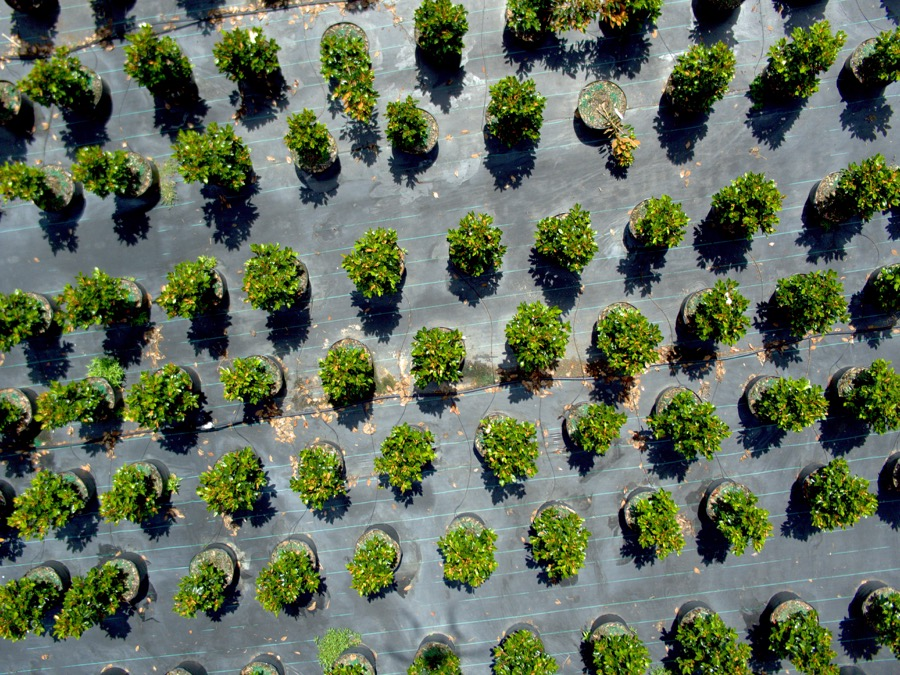
\includegraphics[width=20mm,height=15mm]{figures/input_examples/magnolia_03.jpg}};
\node[sample, xshift=-1.6mm, yshift=1.4mm] at (magback.center) (magmid)
  {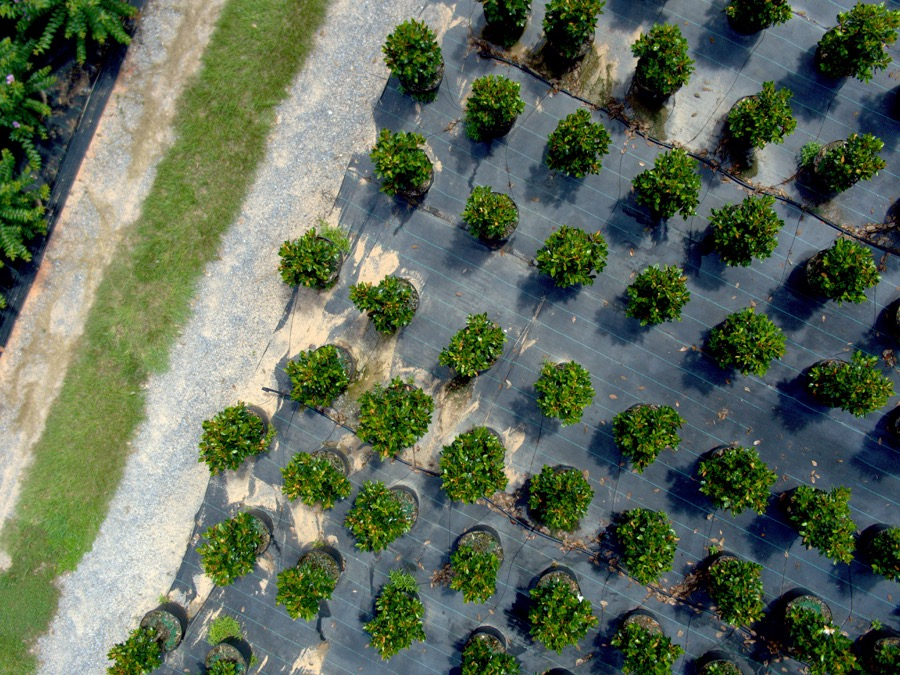
\includegraphics[width=20mm,height=15mm]{figures/input_examples/magnolia_02.jpg}};
\node[sample, xshift=-1.6mm, yshift=1.4mm] at (magmid.center) (mag)
  {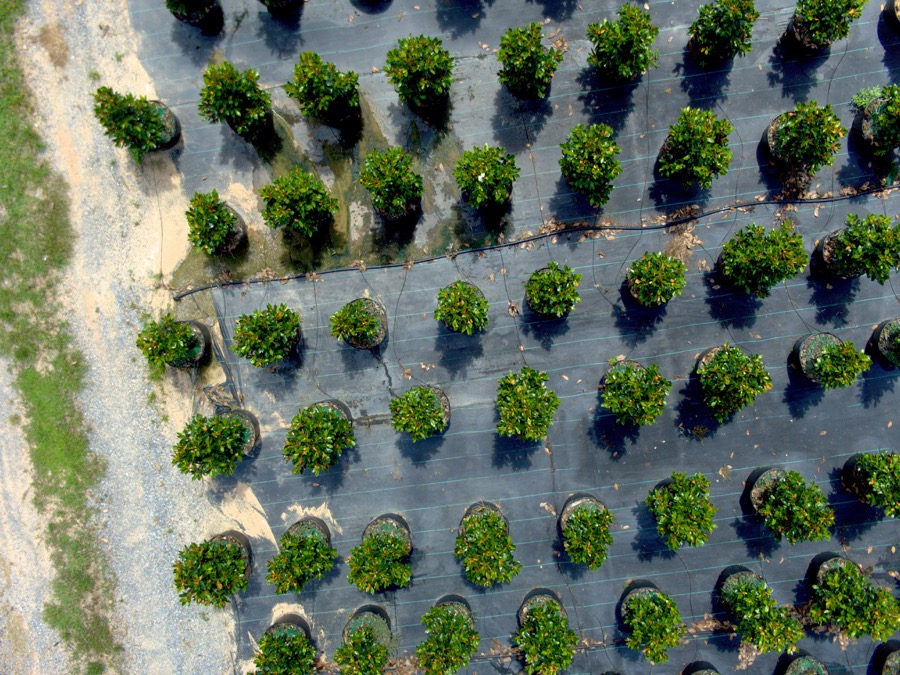
\includegraphics[width=20mm,height=15mm]{figures/input_examples/magnolia_01.jpg}};
\node[fit=(magback)(magmid)(mag), inner sep=.4mm] (magstack) {};
\node[font=\bfseries\scriptsize, above=.7mm of magstack] (maglabel) {Magnolia RGB};

\node[sample, below=8mm of magback] (azaback)
  {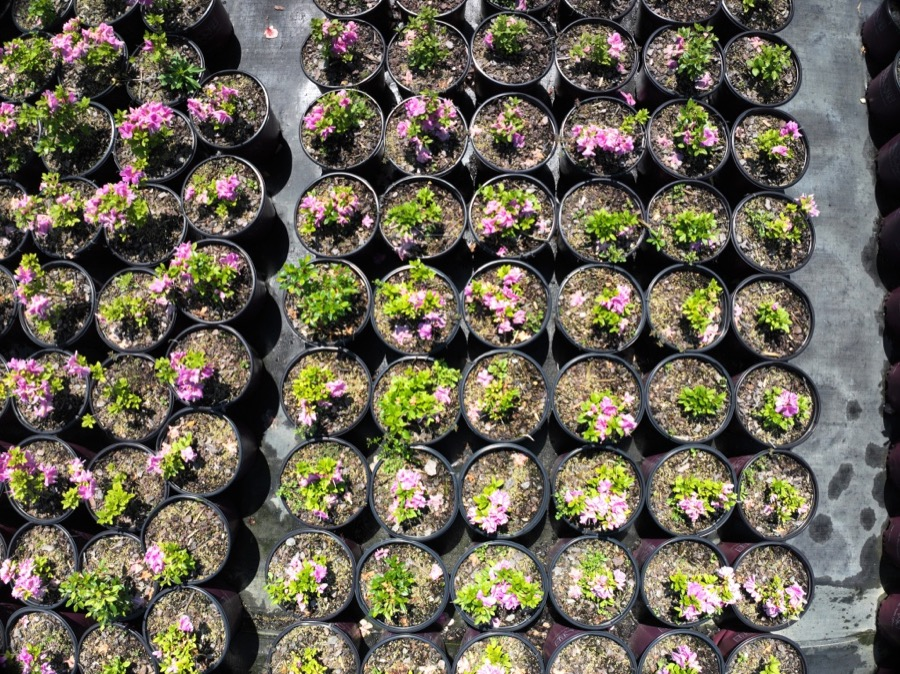
\includegraphics[width=20mm,height=15mm]{figures/input_examples/azalea_03.jpg}};
\node[sample, xshift=-1.6mm, yshift=1.4mm] at (azaback.center) (azamid)
  {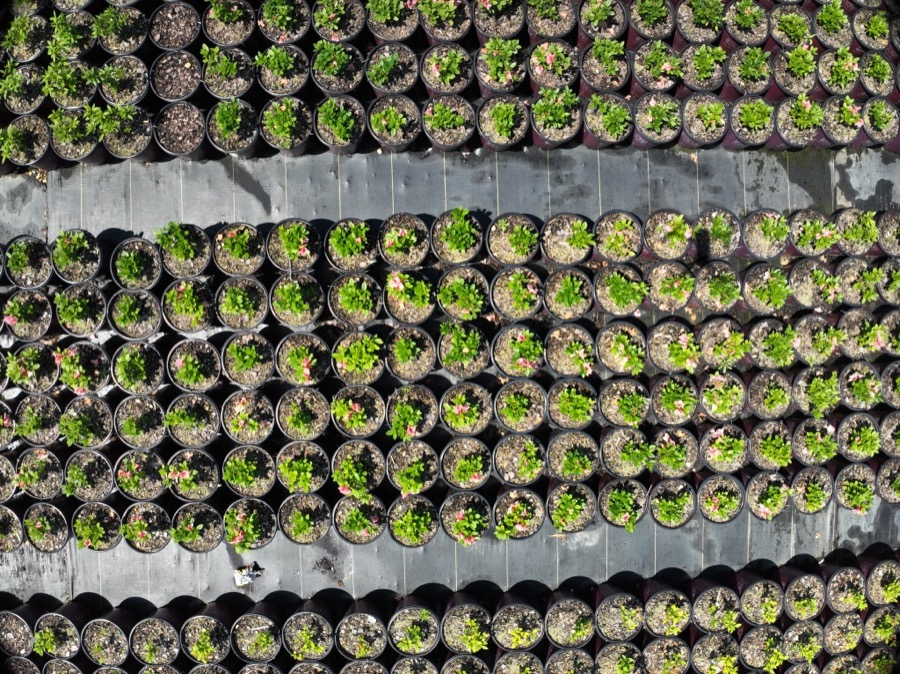
\includegraphics[width=20mm,height=15mm]{figures/input_examples/azalea_02.jpg}};
\node[sample, xshift=-1.6mm, yshift=1.4mm] at (azamid.center) (aza)
  {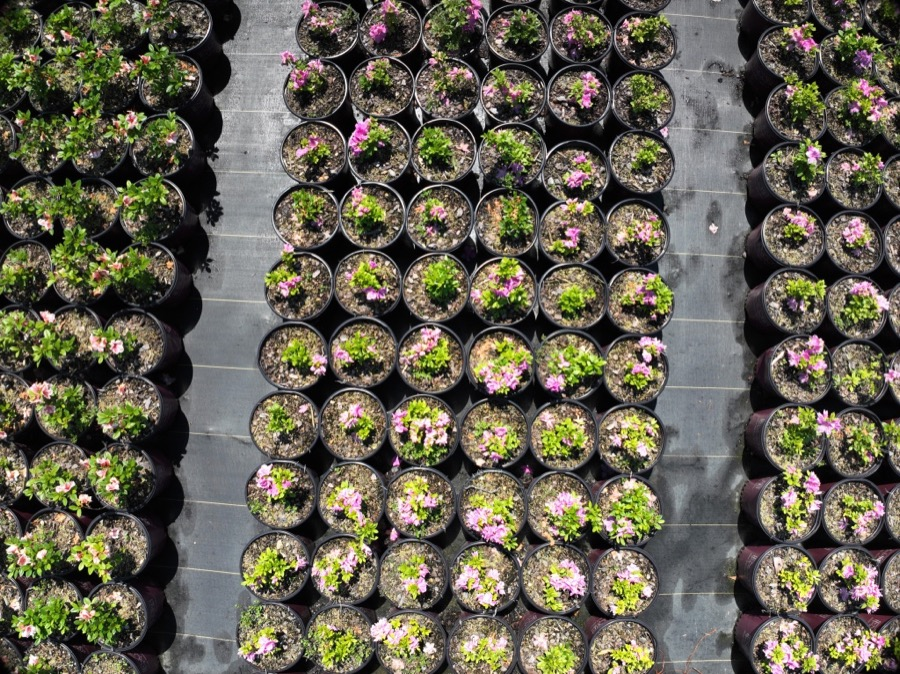
\includegraphics[width=20mm,height=15mm]{figures/input_examples/azalea_01.jpg}};
\node[fit=(azaback)(azamid)(aza), inner sep=.4mm] (azastack) {};
\node[font=\bfseries\scriptsize, above=.7mm of azastack] (azalabel) {Azalea RGB};

\node[prep, right=6mm of $(magstack.east)!0.5!(azastack.east)$] (split)
  {\textbf{Source split}\\train / val / test\\before tiling};
\node[prep, right=5mm of split] (tile)
  {\textbf{Overlapping tiles}\\$s\!\times\!s$, overlap $\alpha$};
\node[evidence, right=5mm of tile] (det)
  {\textbf{Detector evidence}\\confidence $c_t$\\count $n_t$};
\node[outputbox, right=5mm of det, fill=yellow!12, draw=orange!68!black] (labels)
  {\textbf{One-class boxes}\\training / scoring only};

% Row 2: selector, structured inference, and selective output.
\node[select, below=11mm of azastack] (rank)
  {\textbf{Evidence rank}\\$q_t=c_t+\bar n_t$};
\node[select, right=4mm of rank] (allocate)
  {\textbf{Allocate}\\top $K_x$ + explore $K_e$};
\node[select, right=4mm of allocate] (union)
  {\textbf{Budget union}\\$|\mathcal{S}_i|\leq K$};
\node[vlm, right=6mm of union] (adapter)
  {\textbf{VLM adapter}\\SmolVLM2 / Phi\\LLaVA};
\node[vlm, right=4mm of adapter] (schema)
  {\textbf{Schema decoder}\\fixed fields; no\\silent repair};
\node[reliable, right=5mm of schema] (signals)
  {\textbf{Reliability evidence}\\schema, repeats,\\detector agreement};
\node[reliable, right=4mm of signals] (reduce)
  {\textbf{Source reducer}\\overlap-aware\\field fusion};
\node[reliable, right=4mm of reduce] (gate)
  {\textbf{Failure-risk gate}\\validation-fitted\\threshold $\tau^*$};
\node[outputbox, right=4mm of gate, fill=green!8, draw=green!55!black] (accept)
  {\textbf{Accept}\\source record};
\node[outputbox, below=3mm of accept, fill=orange!9, draw=orange!68!black] (review)
  {\textbf{Review}\\abstain / inspect};
\node[outputbox, below=5mm of gate, text width=22mm] (val)
  {\textbf{Validation outcomes}\\observed task failures};

% Boundary-to-boundary paths.
\draw[flow] (magstack.east) -- ++(1.4mm,0) |- ($(split.west)+(0,2mm)$);
\draw[flow] (azastack.east) -- ++(3.0mm,0) |- ($(split.west)+(0,-2mm)$);
\draw[flow] (split.east) -- (tile.west);
\draw[flow] (tile.east) -- (det.west);
\draw[train] (labels.west) -- (det.east);
\coordinate (selectorlane) at ($(rank.north)+(0,2.2mm)$);
\draw[flow] (det.south) |- (selectorlane) -- (rank.north);
\draw[flow] (rank.east) -- (allocate.west);
\draw[flow] (allocate.east) -- (union.west);
\draw[flow] (union.east) -- (adapter.west);
\draw[flow] (adapter.east) -- (schema.west);
\draw[flow] (schema.east) -- (signals.west);
\draw[flow] (signals.east) -- (reduce.west);
\draw[flow] (reduce.east) -- (gate.west);
\node[junction] (gatebranch) at ($(gate.east)+(2mm,0)$) {};
\draw[line width=.7pt, draw=black!78] (gate.east) -- (gatebranch);
\draw[flow] (gatebranch) -- (accept.west);
\draw[flow] (gatebranch) |- (review.west);
\draw[train] (val.north) -- node[right,font=\tiny]{fit on val only} (gate.south);

\begin{scope}[on background layer]
  \node[stage, fit=(maglabel)(magstack)(azalabel)(azastack)(split)(tile)] (stageA) {};
  \node[stage, fit=(det)(labels)] (stageB) {};
  \node[stage, fit=(rank)(allocate)(union), draw=orange!72!black] (stageC) {};
  \node[stage, fit=(adapter)(schema), draw=violet!55!black] (stageD) {};
  \node[stage, fit=(signals)(reduce)(gate)(accept)(review)(val), draw=teal!55!black] (stageE) {};
\end{scope}

% Stage headings are independent of the dashed frames so text never touches a boundary.
\node[font=\bfseries\scriptsize, above=1.1mm of stageA.north]
  {A. Source-safe preparation};
\node[font=\bfseries\scriptsize, above=1.1mm of stageB.north]
  {B. Local evidence};
\node[font=\bfseries\scriptsize, text=orange!55!black, below=1.1mm of stageC.south]
  {C. Budgeted Evidence Selector};
\node[font=\bfseries\scriptsize, text=violet!40!black, below=1.1mm of stageD.south]
  {D. Structured VLM inference};
\node[font=\bfseries\scriptsize, text=teal!38!black, above=1.1mm of stageE.north]
  {E. Selective reliability};
\end{tikzpicture}
}
    \caption{\textbf{OrnaScout overview.} Source images are partitioned before overlapping tiling. A detector evaluates all candidates; equal-budget policies allocate at most $K$ VLM calls. Structured tile records pass through a validation-fitted failure gate and an overlap-aware reducer to form one accepted source record or a review referral. The detector-only path is retained as a controlled baseline. Solid arrows denote deployment computation; dashed arrows denote training or validation-only fitting.}
    \label{fig:architecture}
\end{figure*}

\section{Related Work}
\paragraph{High-resolution aerial detection and counting.}
UAV benchmarks expose persistent variation in scale, density, viewpoint, and background~\cite{du2018uavdt,zhu2018visdrone}. Sliced inference and sparse high-resolution querying preserve small-object detail while avoiding a single severe downsampling step~\cite{akyon2022sahi,yang2022querydet}; one-stage and set-prediction detectors remain strong local evidence producers~\cite{redmon2016yolo,carion2020detr}. Agricultural imagery adds dense repetition, annotation cost, and acquisition shift~\cite{osco2021precision,celikkan2025weedsgalore}. OrnaScout does not replace detection. It uses a detector over candidate tiles and explicitly tests whether a constrained VLM stage adds source-level value beyond deterministic detector aggregation.

\paragraph{Adaptive visual computation.}
The cost of multimodal inference depends on image resolution and visual tokens as well as language-model size. FastVLM, NVILA, and learned token reduction study this accuracy--latency frontier within model architectures~\cite{vasu2025fastvlm,liu2025nvila,zhao2025token}. Active VLM selection similarly motivates spending inference on informative evidence~\cite{safaei2025activevlm}. Our setting instead fixes the number of spatial VLM calls per source image and compares allocation policies under identical cost. The comparison includes random, coordinate-aware spatial, detector-ranked, exploit--explore, and diversity-aware policies rather than assuming that detector ranking is sufficient.

\paragraph{Structured VLM evaluation in specialized domains.}
Contrastive pretraining, caption bootstrapping, frozen-backbone query transformers, and instruction tuning established general visual-language interfaces~\cite{radford2021clip,li2022blip,li2023blip2,dai2023instructblip}. Compact systems such as Phi-3.5-Vision and SmolVLM2 make repeated local inference more plausible~\cite{microsoft2024phi35vision,huggingface2025smolvlm2}. However, plant and aerial evaluations show class-dependent variability and unsupported content~\cite{arshad2025ageval,basak2025aerial,huang2025frisbee}. We therefore evaluate fixed-schema records, strict whole-record validity, hard-negative false positives, repeated-generation consistency, and detector agreement. Free-form fluency is not treated as task correctness.

\paragraph{Domain shift and selective prediction.}
Remote-sensing generalization methods address acquisition and domain changes through adversarial, frequency-based, style-guided, or benchmark-driven evaluation~\cite{ganin2016dann,wang2023uav,alemadi2025shift,danish2024dg,talemi2025stylepro}. Neural confidence can remain miscalibrated under such changes~\cite{guo2017calibration}. Selective classification therefore measures error as coverage changes, while learned rejection and conformal risk control formalize related acceptance decisions under their respective assumptions~\cite{geifman2017selective,geifman2019selectivenet,angelopoulos2024crc}. OrnaScout uses empirical validation calibration and makes no distribution-free guarantee after crop shift. Its gate is compared with raw confidence, strict-schema rejection, detector agreement, and fixed-score baselines at matched operating points.

\paragraph{Precision-agriculture scope.}
UAV sensing and deep learning support inventory and monitoring in precision agriculture~\cite{zhang2012uav,osco2021precision}. Recent ornamental work studies counting under color and domain variation, while agricultural multimodal systems explore domain supervision and localized summaries~\cite{manjunatha2026beyondgreen,awais2025agrogpt,sundaravadivel2026rosai}. The present study is narrower: one-class boxes support inventory-oriented source records, not plant-health or treatment claims. Its primary contribution is the controlled allocation and acceptance of visual evidence under crop shift and finite multimodal computation.

\section{Method}
\subsection{Problem formulation and cost}
Let source image $I_i$ belong to crop domain $d_i$ and occupy valid pixel domain $\Omega_i$. A tiling operator $\mathcal{T}_{s,\alpha}$ produces candidate tiles $\mathcal{T}_i$ with clipped source-coordinate footprints $\Omega_t\subseteq\Omega_i$ and centers $x_t$. Source images are partitioned before tiling. The detector observes every candidate tile; at most $K$ tiles receive VLM inference. The system predicts one record for the complete source image and separately records the union of VLM-inspected footprints. An uninspected region is therefore not treated as an observed negative.

Table~\ref{tab:schema} fixes the roles of all output fields. The four evaluated task fields are annotation-derived inventory surrogates, not independent agronomic labels. Free text, self-reported confidence, and the accept/review decision are audit or system fields and are never scored as biological ground truth.

\begin{table*}[t]
\centering
\wacvtablefont
\caption{Frozen source-record specification. Thresholds and class support are fixed from training data before test evaluation. Annotated coverage is box-derived and must not be described as canopy segmentation.}
\label{tab:schema}
\setlength{\tabcolsep}{4.5pt}
\begin{tabular}{lllll}
\toprule
Field & Allowed value or type & Reference source & Task metric & Gate input \\
\midrule
Plant presence & yes/no & any verified source box & macro-F1 & yes \\
Count & nonnegative estimate and frozen interval & unique source-coordinate boxes & MAE; interval F1 & yes \\
Density class & empty/sparse/moderate/dense & frozen count/valid-area rule & macro-F1 & yes \\
Annotated coverage & none/low/medium/high & clipped box union/valid area & macro-F1; error & yes \\
Visible evidence & text with tile provenance & no independent reference & audit only & no \\
Model confidence & $[0,1]$, self-reported & no independent reference & calibration diagnostic & candidate \\
Decision & accept/review & gate output & risk--coverage & output \\
\bottomrule
\end{tabular}
\end{table*}

For candidate-tile detector cost $C_D$, selected-tile VLM cost $C_V$, and source reduction cost $C_R$, the measured source cost is
\begin{equation}
C(i)=|\mathcal{T}_i|C_D+|\mathcal{S}_i|C_V+C_R,
\qquad |\mathcal{S}_i|\leq K.
\label{eq:cost}
\end{equation}
Selection controls the expensive second term. Rejection occurs after generation and is evaluated as risk control rather than compute saving.

\subsection{Detector evidence and controlled baselines}
A detector trained only on training sources returns source-coordinate detections $\mathcal{D}_t$, their count $n_t=|\mathcal{D}_t|$, and mean retained confidence $c_t$. Confidence thresholding, non-maximum suppression, valid-footprint clipping, and padding removal precede scoring; $c_t=0$ when no detection remains. After this processing, the ranking score is
\begin{equation}
q_t=c_t+\frac{\min(n_t,n_{\max})}{n_{\max}}.
\label{eq:evidence}
\end{equation}
The clipping value $n_{\max}$ and all detector post-processing parameters are chosen on validation sources; crop-stratified saturation rates are reported. Ties are resolved by source-coordinate row, column, then stable tile identifier. Confidence-only, count-only, normalized combined, and spatially deduplicated scores isolate the contribution of each term. The combined score is treated as a heuristic unless a validation comparison supports a stronger interpretation. A detector-only baseline maps fused source-coordinate boxes directly to all derivable output fields and never invokes a VLM.

Training-only hard-negative mining adds reviewed unmatched detector responses from empty training regions. Naturally empty candidates, boundary-aware empty candidates, mined false-positive crops, and verified negative evaluation units are tracked as distinct sets. No validation or test annotation is used to create training negatives. The mining detector, review procedure, and matched-exposure control are reported separately so that any gain is not attributed to evidence allocation.

\subsection{Fixed-budget evidence allocation}
For source $i$, let $K_i=\min(K,|\mathcal{T}_i|)$. The exploit--explore policy assigns $K_e=\min(|\mathcal{T}_i|,\operatorname{round}(\rho K_i))$ slots to exploration and $K_x=K_i-K_e$ to exploitation:
\begin{align}
\mathcal{X}_i &= \operatorname{TopK}_{K_x}(\mathcal{T}_i;q), \\
\mathcal{E}_i &\sim \operatorname{Sample}_{K_e}(\mathcal{T}_i\setminus\mathcal{X}_i), \\
\mathcal{S}_i &= \mathcal{X}_i\cup\mathcal{E}_i.
\label{eq:selector}
\end{align}
If the remaining exploration pool is smaller than $K_e$, every remaining tile is used and the unused slots are returned to exploitation. Sampling uses a seed derived from the study seed, source identifier, policy, budget, and repetition, making the result invariant to manifest order. Stochastic policies are evaluated over repeated seeds; reproducibility from one seed is not treated as robustness. Candidate manifests are shared by all policies, and whether budget sets are nested is declared before evaluation.

Equal-budget controls include random sampling, confidence top-$K$, count top-$K$, combined-score top-$K$, and two geometry-aware policies. Spatial selection applies farthest-point sampling to normalized tile centers $x_t$, while diversity-aware exploration selects remaining tiles using distance from the exploited set and detector-score uncertainty. Ground-truth routing and shuffled detector scores are diagnostic controls only. The method does not assume that exploit--explore is uniformly optimal; policy selection is frozen from validation utility--risk trade-offs.

\subsection{Source-level evidence diagnostics}
Let $\mathcal{B}_i$ be the one-class source annotations and $v(b,t)$ the intersection area between box $b$ and tile footprint $\Omega_t$, divided by the unclipped area of $b$. At visibility threshold $\eta$, source evidence recall is
\begin{equation}
R_{\mathrm{evid}}(i)=\frac{1}{|\mathcal{B}_i|}
\sum_{b\in\mathcal{B}_i}\mathbb{1}\!\left[
\max_{t\in\mathcal{S}_i}v(b,t)\geq\eta\right].
\label{eq:evidence-recall}
\end{equation}
Each source box receives credit at most once. Spatial coverage and overlap redundancy are
\begin{align}
C_{\mathrm{sp}}(i)&=\frac{|\bigcup_{t\in\mathcal{S}_i}\Omega_t|}{|\Omega_i|}, \\
D_{\mathrm{red}}(i)&=
\frac{\sum_{t\in\mathcal{S}_i}|\Omega_t|}
{|\bigcup_{t\in\mathcal{S}_i}\Omega_t|}-1.
\label{eq:spatial}
\end{align}
For empty sources, $R_{\mathrm{evid}}$ is undefined and excluded from the source-macro evidence-recall mean; negative-source behavior is reported separately. All footprints are clipped to $\Omega_i$, padding is excluded, and empty selected unions receive zero spatial coverage with redundancy marked undefined. Boundary truncation records covered instances with maximum visible fraction in $[\eta,.98)$. We report both negative retention (selected verified-negative candidates divided by all verified-negative candidates) and selected-negative fraction (selected verified-negative candidates divided by all selected candidates); neither is called recall without its denominator. These diagnostics measure available evidence, not task correctness.

\subsection{Structured multimodal inference}
Each selected tile and one frozen instruction are passed to a model-specific adapter. The current implementation uses prompt-only formatting followed by post-generation JSON extraction and validation; it is not grammar-constrained decoding. The frozen prompt, schema version, native image processor, generation parameters, raw output, and parser version are recorded. The parser records malformed output without silently repairing task fields. For generation $z$, constraint satisfaction and strict validity are distinct:
\begin{align}
s_{\mathrm{constr}}(z)&=\frac{1}{J}\sum_{j=1}^{J}\mathbb{1}[g_j(z)=1], \\
v_{\mathrm{schema}}(z)&=\prod_{j=1}^{J}\mathbb{1}[g_j(z)=1].
\label{eq:schema}
\end{align}
With $R>1$ generations, repeat consistency averages modal agreement over the four evaluated categorical fields $\mathcal{F}=\{\text{presence, count interval, density, annotated coverage}\}$:
\begin{equation}
s_{\mathrm{rep}}(t)=\frac{1}{|\mathcal{F}|}
\sum_{k\in\mathcal{F}}
\frac{\max_v\sum_{r=1}^{R}\mathbb{1}[z_{t,r,k}=v]}{R}.
\label{eq:consistency}
\end{equation}
Malformed or missing fields are retained as explicit disagreement. When $R=1$, repeat consistency is unavailable rather than set to one. The delivered tile prediction rule (first generation or frozen consensus) is declared before evaluation. Agreement is a stability diagnostic, not evidence of correctness. Detector agreement $s_{\mathrm{det}}$ compares VLM presence and count interval with fused detector evidence and is not treated as independent verification.

\subsection{Overlap-aware source reduction}
Detector boxes from all candidate tiles are projected to source coordinates and fused once using a validation-selected overlap threshold. Selected-tile VLM records annotate only their inspected footprints. Presence follows a frozen false-positive rule; count uses coordinate-aware fused instances; density uses count per valid source area; and annotated coverage uses the union of clipped fused boxes divided by valid source area. Categorical VLM fields use frozen reliability-weighted voting only where they are not deterministic functions of the fused boxes. Field conflicts and the uninspected-area fraction are retained as reducer features. The reducer returns a source record $\tilde y_i$ and reliability vector
\begin{equation}
u_i=[\bar v_{\mathrm{schema}},\bar s_{\mathrm{constr}},
\bar s_{\mathrm{rep}},\bar s_{\mathrm{det}},s_{\mathrm{conflict}},
s_{\mathrm{support}}].
\label{eq:sourcefeatures}
\end{equation}
If no valid VLM record remains, or if required evidence is unobserved under the frozen rule, the source is referred for review rather than relabeled empty. Reducer rules, overlap threshold, and field weights are frozen on validation sources.

\subsection{Validation-only selective decision}
A transparent fixed baseline averages the available reliability signals after orienting each so that larger is safer. The learned gate estimates source-record error probability $\hat r_i=h(u_i)$. To avoid fitting and thresholding on the same outcomes, source-grouped cross-fitting produces out-of-fold validation risks. For predeclared target risk $\epsilon$, the threshold is
\begin{equation}
\tau^*=\max_{\tau\in\mathcal{Q}_{\mathrm{val}}}\left\{\tau:
|A_\tau|\geq n_{\min},\quad
\frac{\sum_{i\in A_\tau}e_i}{|A_\tau|}\leq\epsilon\right\},
\label{eq:threshold}
\end{equation}
where $A_\tau=\{i:\hat r_i\leq\tau\}$, $e_i=1$ when any required source-level task field is incorrect, $\mathcal{Q}_{\mathrm{val}}$ is the frozen set of out-of-fold validation scores, and $n_{\min}$ is a predeclared minimum accepted count. If no threshold satisfies both constraints, the target is declared unattained; an empty accepted set is never reported as zero risk. Threshold ties use the highest-coverage rule followed by the lower-risk rule. After features and $\tau^*$ are frozen, the gate is refit on all validation sources and evaluated once on test sources. Records with $\hat r_i\leq\tau^*$ are accepted; all others are referred for review. This is empirical validation thresholding, not probability calibration or a distribution-free guarantee after crop shift.

\begin{algorithm}[t]
\caption{Fixed-budget source inference with selective review}
\label{alg:ornascout}
\begin{algorithmic}[1]
\Require $I_i$, tiler $(s,\alpha)$, detector/post-processing $f_D$, VLM $f_V$, prompt/schema $p$, repeats $R$, budget $K$, seed, frozen policy $\pi$, reducer $A$, gate $h_{\tau^*}$
\Ensure Source record $\tilde y_i$, decision $a_i$, tile audit trail $L_i$, and stage-cost ledger $G_i$
\State Initialize $L_i,G_i$; $\mathcal{T}_i\gets\mathcal{T}_{s,\alpha}(I_i)$ with coordinates and valid footprints
\ForAll{$t\in\mathcal{T}_i$}
  \State $\mathcal{D}_t\gets f_D(t)$; filter, clip, cache evidence, and update $G_i$
\EndFor
\State $\mathcal{S}_i\gets\pi(\mathcal{T}_i,\{\mathcal{D}_t\},\min(K,|\mathcal{T}_i|),\mathrm{seed}_i)$
\State $\mathcal{Z}_i\gets\emptyset$
\ForAll{$t\in\mathcal{S}_i$}
  \For{$r=1$ to $R$}
    \State Store raw $o_{t,r}\gets f_V(t,p)$; parse or mark malformed; update $L_i,G_i$
  \EndFor
  \State $\mathcal{Z}_i\gets\mathcal{Z}_i\cup\{(t,\Omega_t,o_{t,1:R})\}$
\EndFor
\State $(\tilde y_i,u_i)\gets A(\mathcal{Z}_i,\{(t,\Omega_t,\mathcal{D}_t):t\in\mathcal{T}_i\})$
\State $a_i\gets\mathrm{accept}$ if $h(u_i)\leq\tau^*$, else $\mathrm{review}$
\State \Return $\tilde y_i,a_i,L_i,G_i$
\end{algorithmic}
\end{algorithm}

\section{Experimental Design}
\subsection{Corpus, annotations, and audit}
The frozen snapshot contains 418 source images: 297 Magnolia and 121 Azalea. Five zero-width annotation rows are rejected without modifying the reviewed labels, leaving 29,842 one-class plant boxes (15,644 Magnolia and 14,198 Azalea). Three reviewed Azalea sources contain no instances and are retained as source-level negatives; one unmatched RGB frame is excluded. With $1024\!\times\!1024$ tiles, $.25$ overlap, and minimum box visibility $.5$, preparation yields 14,630 tiles, including 1,328 boundary-aware empty candidates.

\begin{table}[t]
\centering
\wacvtablefont
\caption{Frozen corpus and source-safe split. Human-audit and detector columns remain blocked until their artifacts are verified.}
\label{tab:data}
\setlength{\tabcolsep}{3.5pt}
\begin{tabular}{lrrrrr}
\toprule
Crop & Sources & Boxes & Train/Val/Test & Audit & Det. rec. \\
\midrule
Magnolia & 297 & 15,644 & \pendingcell & \pendingcell & \pendingcell \\
Azalea & 121 & 14,198 & \pendingcell & \pendingcell & \pendingcell \\
\midrule
Total & 418 & 29,842 & 302/58/58 & \pendingcell & \pendingcell \\
\bottomrule
\end{tabular}
\end{table}

A frozen human audit stratifies by crop, source, normalized box size, image boundary, annotation density, and negative status. The final report will state sample size, reviewer count, agreement, adjudication, and exclusions. Exact and perceptual duplicate checks operate at source level; source, sequence, flight, or row identifiers are grouped when metadata permit. Split and manifest hashes are recorded before model evaluation.

\subsection{Observed domain shift}
Azalea contains a higher median annotated count per source than Magnolia and a smaller median normalized box area. Appearance and green-fraction distributions also differ. Figure~\ref{fig:domainshift} describes these measured marginals before model fitting; it motivates directed evaluation but is not treated as causal proof of transfer error.

\begin{figure*}[t]
    \centering
    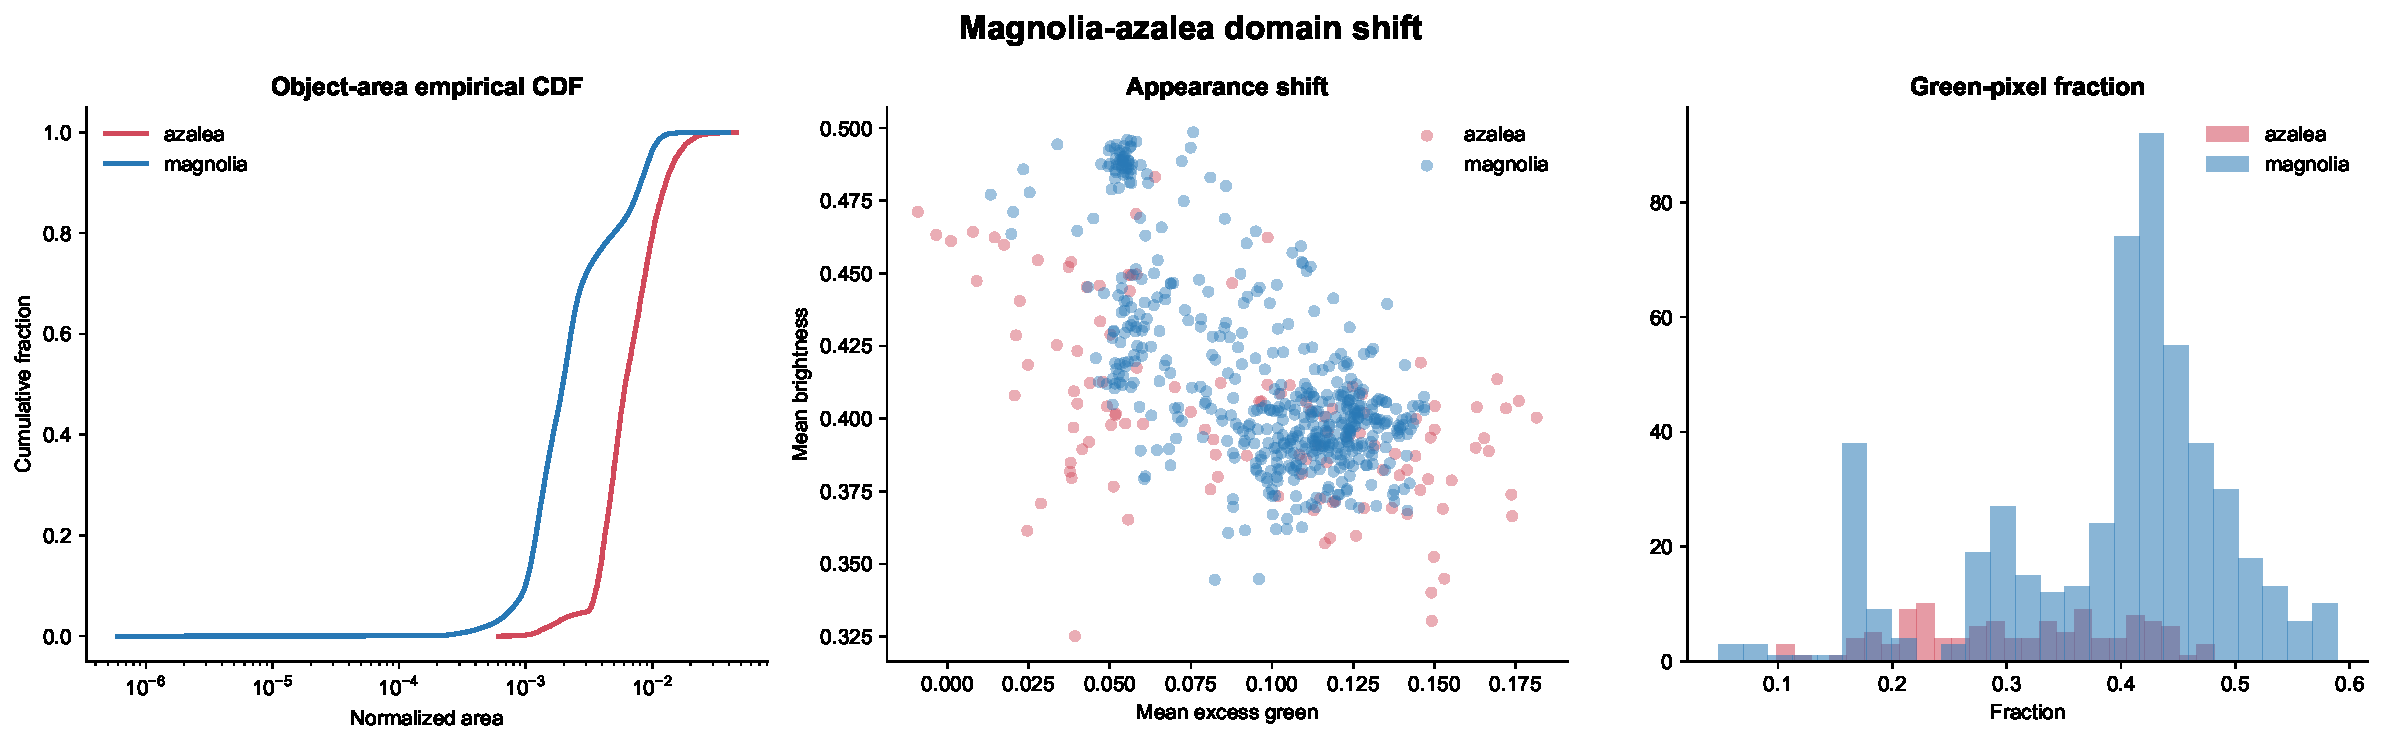
\includegraphics[width=\textwidth]{figures/cross_crop_shift.pdf}
    \caption{\textbf{Measured Magnolia--Azalea shift.} Object geometry uses valid source boxes; appearance statistics are computed once per source. No model prediction enters the figure. The corresponding directed transfer results are reported separately.}
    \label{fig:domainshift}
\end{figure*}

\subsection{Tasks and source-level targets}
Presence is positive when a source contains at least one verified instance. Count is evaluated continuously by mean absolute error and categorically using intervals fitted on training sources only. Density and annotated coverage use training-only thresholds with adequate support in every evaluated class; otherwise they remain continuous or diagnostic outcomes. The primary endpoint is strict source-record correctness: all required inventory fields must be correct. Per-field macro-F1, count error, and coverage error are secondary endpoints. A malformed record is incorrect rather than silently repaired.

\subsection{Directed evaluation protocols}
We evaluate Magnolia$\rightarrow$Magnolia (M$\rightarrow$M), Azalea$\rightarrow$Azalea (A$\rightarrow$A), M$\rightarrow$A, A$\rightarrow$M, and crop-stratified pooled training. Here transfer refers explicitly to every fitted component: detector, ranking parameters, reducer, and gate. The VLM checkpoint remains frozen. Target-crop test labels are used only for final scoring. Tile parameters, prompt, schema, risk target, and all component choices are frozen without target-test feedback. Method comparisons on the same target sources use paired resampling; differences between distinct Magnolia and Azalea test sets are domain gaps and are not called paired effects.

\subsection{Controlled systems and baselines}
The primary VLM is chosen on validation evidence before test scoring. SmolVLM2-500M, SmolVLM2-2.2B, Phi-3.5-Vision, and LLaVA-1.5-7B form a secondary model ladder. All VLMs receive the same source tiles, semantic prompt, output schema, generation-token cap, and stopping rule. Because native image processors differ, processed tensor resolution and visual-token count are recorded rather than described as identical visual input.

The system comparison includes: (i) detector-only source aggregation; (ii) deterministic detector-derived inventory rules; (iii) one whole-image downsampled VLM input; (iv) uniformly tiled VLM inference at budget $K$; and (v) detector-routed VLM inference with and without selective review. Routing policies are random, true coordinate-aware spatial selection, confidence top-$K$, count top-$K$, normalized combined top-$K$, exploit--explore, and diversity-aware exploration. Shuffled scores and GT-oracle routing are diagnostic controls only.

Reliability baselines are raw VLM confidence, strict-schema rejection, detector agreement, an equal-weight fixed score, and the cross-fitted learned gate. Comparisons are made at matched coverage and at one validation-declared target risk.

\subsection{Metrics, uncertainty, and efficiency}
For test sources ordered by increasing predicted risk, let $e_{(j)}$ indicate strict source-record error. Selective risk and area under the risk--coverage curve are
\begin{equation}
R_m=\frac{1}{m}\sum_{j=1}^{m}e_{(j)},\qquad
\mathrm{AURC}=\frac{1}{N}\sum_{m=1}^{N}R_m.
\label{eq:aurc}
\end{equation}
We also report coverage at the declared target risk, observed accepted risk, false acceptance on verified negative sources, accepted-source count, and review rate. Routing diagnostics are evidence recall, spatial coverage, overlap redundancy, boundary truncation, negative retention, and selected-negative fraction.

All intervals use source-clustered bootstrap resampling, or a higher acquisition group when flight/block metadata show dependence. Policy and model comparisons on shared target sources use paired bootstrap differences; marginal interval overlap is not used as a significance test. Stochastic routing uses order-invariant per-source seeds and repeated runs. Hyperparameters and policy selection use validation data only.

Efficiency is measured from source decoding to final decision: tiling, detector inference, selection, image preparation/transfer, VLM generation, parsing, gating, and reduction. Timings use synchronized devices, declared batching, warm-up, repeated source-level measurements, and explicit model-loading inclusion/exclusion. We report mean and p95 source latency, throughput, peak host and accelerator memory, model-loading memory, VLM calls and generations per source, and expected review workload on named hardware and software revisions. Per-tile p95 values are never multiplied to approximate source-level p95.

\subsection{Numerical provenance}
Every table and figure is generated from immutable artifacts recording the Git commit, command, dataset and split hashes, model revision, checkpoint hash, seed, hardware, software environment, and output hash. Values in this working draft remain pending until that record is complete. The held-out test set is evaluated once after the primary configuration is frozen.

\section{Results}
\paragraph{Release rule.}
Only values generated from frozen artifacts enter the final manuscript. Red dashes in this working revision identify required experiments; they are not zero values and must not be estimated manually.

\subsection{Data integrity and detector evidence}
The final version will first establish that source partitions are disjoint, that negative sources were reviewed, and that detector evidence is characterized by crop, object scale, and annotation density. Table~\ref{tab:data} will include the completed human-audit and detector-recall entries. Hard-negative mining will remain a supporting detector refinement unless its matched artifacts establish a reproducible gain.

\draftnote{Insert duplicate/leakage audit, human-review agreement, detector M$\rightarrow$M, A$\rightarrow$A, M$\rightarrow$A, and A$\rightarrow$M results.}

\subsection{Equal-budget evidence allocation}
Table~\ref{tab:allocation} is designed to report the complete policy trade-off rather than select a winner from one metric. The final analysis will compare paired source-level differences against combined top-$K$ and coordinate-aware spatial selection. A policy will be described as preferable only for an explicitly stated operating objective.

\begin{table*}[t]
\centering
\wacvtablefont
\caption{Equal-budget source-level comparison at the validation-selected primary configuration. Exact is strict source-record accuracy; AURC is lower-is-better. All intervals and paired comparisons are clustered by source.}
\label{tab:allocation}
\setlength{\tabcolsep}{5pt}
\begin{tabular}{lccccccc}
\toprule
Policy & Exact$\uparrow$ & Evid. rec.$\uparrow$ & Spatial cov.$\uparrow$ & Redund.$\downarrow$ & Hard-neg.$\uparrow$ & AURC$\downarrow$ & p95 ms$\downarrow$ \\
\midrule
Random & \pendingcell & \pendingcell & \pendingcell & \pendingcell & \pendingcell & \pendingcell & \pendingcell \\
Spatial (2D) & \pendingcell & \pendingcell & \pendingcell & \pendingcell & \pendingcell & \pendingcell & \pendingcell \\
Confidence top-$K$ & \pendingcell & \pendingcell & \pendingcell & \pendingcell & \pendingcell & \pendingcell & \pendingcell \\
Count top-$K$ & \pendingcell & \pendingcell & \pendingcell & \pendingcell & \pendingcell & \pendingcell & \pendingcell \\
Combined top-$K$ & \pendingcell & \pendingcell & \pendingcell & \pendingcell & \pendingcell & \pendingcell & \pendingcell \\
Exploit--explore & \pendingcell & \pendingcell & \pendingcell & \pendingcell & \pendingcell & \pendingcell & \pendingcell \\
Diversity-aware & \pendingcell & \pendingcell & \pendingcell & \pendingcell & \pendingcell & \pendingcell & \pendingcell \\
\bottomrule
\end{tabular}
\end{table*}

\begin{figure}[t]
\centering
\fbox{\parbox[c][36mm][c]{0.93\columnwidth}{\centering
\textbf{Pending artifact-generated policy Pareto plot}\\[2mm]
Source utility versus accepted risk; marker annotations report budget and latency.}}
\caption{\textbf{Allocation Pareto frontier.} The final figure will show paired source-level utility, risk, and compute for equal-budget routing policies.}
\label{fig:pareto}
\end{figure}

\subsection{Does the VLM add source-level value?}
Table~\ref{tab:vlmvalue} directly addresses the necessity of multimodal inference. Detector-only and deterministic aggregation are primary controls, not secondary ablations. The VLM claim will be retained only if source-level utility or selective behavior improves at a reported cost.

\begin{table*}[t]
\centering
\wacvtablefont
\caption{Source-level system comparison on the frozen pooled test protocol. Count error is reported continuously; FAR is false acceptance on verified negative sources.}
\label{tab:vlmvalue}
\setlength{\tabcolsep}{4.5pt}
\begin{tabular}{lcccccccc}
\toprule
System & Pres. F1 & Count err.$\downarrow$ & Dens. F1 & Cov. F1 & Exact$\uparrow$ & FAR$\downarrow$ & Review$\downarrow$ & p95 ms$\downarrow$ \\
\midrule
Detector only & \pendingcell & \pendingcell & \pendingcell & \pendingcell & \pendingcell & \pendingcell & -- & \pendingcell \\
Detector + rules & \pendingcell & \pendingcell & \pendingcell & \pendingcell & \pendingcell & \pendingcell & -- & \pendingcell \\
Whole-image VLM & \pendingcell & \pendingcell & \pendingcell & \pendingcell & \pendingcell & \pendingcell & \pendingcell & \pendingcell \\
Uniform tiled VLM & \pendingcell & \pendingcell & \pendingcell & \pendingcell & \pendingcell & \pendingcell & \pendingcell & \pendingcell \\
OrnaScout, no gate & \pendingcell & \pendingcell & \pendingcell & \pendingcell & \pendingcell & \pendingcell & -- & \pendingcell \\
OrnaScout + gate & \pendingcell & \pendingcell & \pendingcell & \pendingcell & \pendingcell & \pendingcell & \pendingcell & \pendingcell \\
\bottomrule
\end{tabular}
\end{table*}

\subsection{Directed crop transfer}
Table~\ref{tab:transfer} reports each training--test direction separately. The final analysis will give the paired drop from the corresponding in-domain reference and decompose it into detector miss, routing miss, structured-prediction error, and rejection behavior. Object scale and density are diagnostic strata, not post-hoc causal proof.

\begin{table}[t]
\centering
\wacvtablefont
\caption{Directed source-level transfer. Each cell reports the primary utility with source-clustered 95\% interval; $\Delta$ is the paired drop from the corresponding in-domain reference.}
\label{tab:transfer}
\setlength{\tabcolsep}{5pt}
\begin{tabular}{lcccc}
\toprule
Train & Test M & $\Delta$ & Test A & $\Delta$ \\
\midrule
Magnolia & \pendingcell & -- & \pendingcell & \pendingcell \\
Azalea & \pendingcell & \pendingcell & \pendingcell & -- \\
Pooled & \pendingcell & \pendingcell & \pendingcell & \pendingcell \\
\bottomrule
\end{tabular}
\end{table}

\subsection{Selective reliability and review burden}
Figure~\ref{fig:riskcoverage} will compare raw VLM confidence, strict-schema rejection, detector agreement, fixed-score ranking, and the cross-fitted learned gate. The operating point is selected from out-of-fold validation predictions before test scoring. The corresponding table reports coverage, accepted risk, negative-source false acceptance, accepted source count, and human-review rate.

\begin{figure}[t]
\centering
\fbox{\parbox[c][39mm][c]{0.93\columnwidth}{\centering
\textbf{Pending artifact-generated risk--coverage curves}\\[2mm]
Raw confidence, schema-only, detector agreement, fixed score, learned gate; validation-selected operating point marked.}}
\caption{\textbf{Held-out selective reliability.} Curves and intervals use source-level outcomes; lower risk at negligible coverage is not treated as operational success.}
\label{fig:riskcoverage}
\end{figure}

\begin{table}[t]
\centering
\wacvtablefont
\caption{Held-out reliability at the predeclared target-risk operating point.}
\label{tab:reliability}
\setlength{\tabcolsep}{3.4pt}
\begin{tabular}{lccccc}
\toprule
Score & AURC$\downarrow$ & Cov.$\uparrow$ & Risk$\downarrow$ & FAR$\downarrow$ & Accepted \\
\midrule
Raw confidence & \pendingcell & \pendingcell & \pendingcell & \pendingcell & \pendingcell \\
Strict schema & \pendingcell & \pendingcell & \pendingcell & \pendingcell & \pendingcell \\
Detector agreement & \pendingcell & \pendingcell & \pendingcell & \pendingcell & \pendingcell \\
Fixed score & \pendingcell & \pendingcell & \pendingcell & \pendingcell & \pendingcell \\
Learned gate & \pendingcell & \pendingcell & \pendingcell & \pendingcell & \pendingcell \\
\bottomrule
\end{tabular}
\end{table}

\subsection{Efficiency and failure analysis}
End-to-end timing will separate tiling, detection, selection, image transfer, VLM generation, parsing, gating, and reduction. The failure audit uses a frozen, crop-balanced, size-balanced source sample. Categories are annotation issue, detector miss, routing miss, boundary truncation, malformed schema, task error, unsupported positive, reduction conflict, gate false accept, gate false reject, and correct abstention.

\draftnote{Insert named-hardware efficiency table, failure counts with denominators and agreement, and frozen-rule qualitative panels.}

\section{Discussion and Limitations}
OrnaScout addresses a systems question: how should a limited multimodal budget be allocated and accepted when source images are much larger than a compact VLM's visual context? The answer need not be one universally dominant selector. Detector ranking, spatial diversity, and negative evidence optimize different objectives; the useful result is the measured operating frontier and the conditions under which each policy improves source-level utility or selective risk.

The VLM stage is similarly treated as an empirical hypothesis. Presence, count, density, and coverage can often be derived from detections, so detector-only and deterministic aggregation are necessary controls. Structured VLM inference is justified only if it adds source-level utility, auditable evidence, or better selective behavior at a transparent computational and review cost. Otherwise, the simpler detector system is the appropriate conclusion.

Several limitations bound the study. The corpus contains two ornamental crop domains and is imbalanced in source count, annotation density, and object scale. One-class boxes support inventory-oriented outcomes but not health, stress, quality, mortality, yield, or treatment recommendations. The selector inherits detector misses; exploration can expose overlooked regions but cannot guarantee recovery. Empirical calibration can fail after severe target shift and does not provide distribution-free risk control. Source-level review also incurs human cost, which must be reported alongside machine latency. Finally, private imagery can support a controlled systems study but is not a dataset contribution unless release rights, documentation, and access are established.

The intended use is decision support. Accepted records summarize visual evidence under a declared protocol; review referrals identify sources for human inspection. Neither path replaces agronomic judgment.

\section{Conclusion}
This revision formulates high-resolution UAV nursery analysis as fixed-budget, source-level evidence allocation with selective review. The completed paper will establish whether structured VLM evidence adds value beyond detector-only aggregation, quantify directed crop transfer, and report the utility--risk--compute frontier of equal-budget policies. \pending{Replace with the final artifact-verified finding and bounded implication before submission.}


% Keep all method and result figures ahead of the bibliography without
% forcing an otherwise unnecessary blank column or page.
\FloatBarrier
{\small
\bibliographystyle{ieeenat_fullname}
\bibliography{references}
}
\end{document}
